\documentclass[8pt]{beamer}

\usepackage{amsfonts}
\usepackage{subfiles}
\usepackage[T2A]{fontenc}
\usepackage[utf8]{inputenc}
\usepackage[russian]{babel}

\usepackage{amsmath, amsfonts, amssymb, amsthm, mathtools, mathrsfs}
\usepackage{wasysym, dsfont}
\usepackage{graphicx}
\usepackage{float}
\usepackage{wrapfig}

\usepackage{caption}
\usepackage{subcaption}
% \usepackage{subfigure}

\usepackage{multicol}
\DeclareMathOperator*{\argmax}{\arg\!\max}
\DeclareMathOperator*{\argmin}{\arg\!\min}

\mode<presentation>
{
	\usetheme{boxes}
	\beamertemplatenavigationsymbolsempty
	
	\setbeamertemplate{footline}[page number]
	\setbeamersize{text margin left=1.5em, text margin right=2.0em}
}
\newcommand\blfootnote[1]{%
	\begingroup
	\renewcommand\thefootnote{}\footnote{#1}%
	\addtocounter{footnote}{-1}%
	\endgroup
}


\title[]{Ускорение семплирования из диффузионных моделей с использованием состязательных сетей}
\author{Охотников Никита Владимирович}
\institute{МФТИ}
\date{2023}


\begin{document}

\begin{frame}
  \titlepage
\end{frame}


\begin{frame}
	\frametitle{Цели исследования}
	
	\begin{columns}
		\begin{column}{0.9\textwidth}
	
			\begin{block}{Цель}
				\smallskip
			Модификацировать классическую диффузионную модель для существенного ускорения процесса семплирования
			\end{block}	
		
			\bigskip
		
			\begin{block}{Задача}
					\smallskip
				Проанализировать способы моделирования мультимодального распределения в обратном диффузионном процессе
			\end{block}	
		
			\bigskip
			
			\begin{block}{Предлагается}
				\smallskip
				Использовать неявную генеративную модель -- состязательну сеть на каждом шаге диффузионного процесса
			\end{block}	
		
			\bigskip
		
			\begin{block}{Необходимо}
				\smallskip
				Рассмотреть различные постановки минимизацонной задачи для используемой модели
			\end{block}	

	     \end{column}
	\end{columns}


\end{frame}




	%\setlength{\footskip}{1.8cm}
\begin{frame}
	\frametitle{Неявное моделирование обратного диффузионного процесса}


	\begin{columns}
		\begin{column}{0.5\textwidth}
			\begin{block}{Диффузионный процесс}
				\begin{itemize}
				
					\item Прямой: 
					\begin{equation*}
					q(\textbf{x}_t|\textbf{x}_{t-1}) = \mathcal{N}(\textbf{x}_t; \textbf{x}_{t-1}\sqrt{1-\beta_t}, \beta_t 	\textbf{I})
					\end{equation*}
					где $t = \overline{0,T}$, $\textbf{x}_0$ -- семпл из исходного распределения, $\textbf{x}_t$ -- семпл на шаге $t$, $\beta_t\in (0,1)$\\
					
					\item Обратный: 
					\begin{equation*}
					p_\theta(\textbf{x}_{t-1}|\textbf{x}_t)\!\! \underset{\text{T} \gg 1}{ \approx}\!\!\! \mathcal{N}(\textbf{x}_{t-1};\mu_\theta(\textbf{x}_t,t), \Sigma_\theta(\textbf{x}_t, t))
					\end{equation*}
			
				\end{itemize}
			\end{block}		
		\end{column}
		
		\begin{column}{0.55\textwidth} 
				\begin{figure}[h!]
						\begin{flushright}
							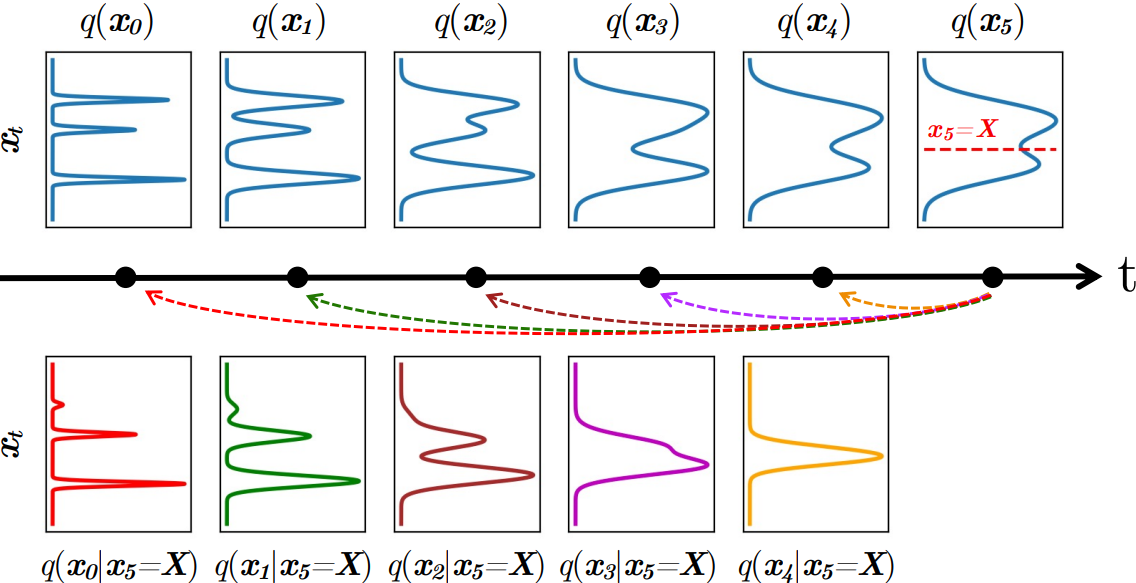
\includegraphics[width=0.97\textwidth]{figures/distributions.png}
						\end{flushright}	
				\end{figure}
	
		\end{column}
	\end{columns}


\begin{columns}
	\begin{column}{0.4\textwidth}
		
		\begin{block}{Основные предположения}
			
			\begin{itemize}	
				\item Марковость обратного процесса
				\item Нормальность и следовательно унимодальность $p_\theta(\textbf{x}_{t-1}|\textbf{x}_t)$
			\end{itemize}
		
		\end{block}
	
	\end{column}
	
	\begin{column}{0.57\textwidth}  
			\begin{block}{Предложение}
				\begin{itemize}
					\item Использовать неявную модель для восстановления распределения
				\end{itemize}
			\end{block}	
		\begin{block}{Мотивация}
			\begin{itemize}
				\item Моделирование мультимодального распределения для существенного уменьшения T
			\end{itemize}
		\end{block}	
	\end{column}
\end{columns}
			\blfootnote{\url{https://doi.org/10.48550/arxiv.2112.07804}}
\end{frame}



\begin{frame}
		\frametitle{Диффузионная модель}
		\begin{block}{Описание}
		В основе модели лежит постепенное добавление случайного нормального шума с коэффициентом $\beta_t\in (0,1)$ в семпл $\textbf{x}_0$ из исходного распределения в прямом процессе и постепенное восстановление распределения в обратном. 
		\end{block}
	\begin{columns}
		
		\begin{column}{0.5\textwidth}
			\begin{block}{Прямой процесс}
				\begin{equation*}
					q(\textbf{x}_t|\textbf{x}_{t-1}) = \mathcal{N}(\textbf{x}_t; \textbf{x}_{t-1}\sqrt{1-\beta_t}, \beta_t 	\textbf{I})
				\end{equation*}
					где $t = \overline{0,T}$, $\textbf{x}_t$ -- семпл на шаге $t$.
				В таком случае, принимая $\alpha_t  = 1 - \beta_t,~\overline{\alpha_t} = \prod_{i=1}^t \alpha_i$ можно записать:
				\begin{equation*}
					q(\textbf {x}_t | \textbf{x}_0 ) = \mathcal{N} (\textbf{x}_t; \sqrt{\overline{\alpha_t}} \textbf{x}_0, (1-\overline{\alpha_t}) \textbf{I})
				\end{equation*}
				Таким образом, при достаточно больших $T$ со сколь угодно большой точностью $\textbf{x}_T\sim \mathcal{N}(0, \textbf{I})$, а значит обратный процесс начинается с нормального шума.				
			\end{block}  	 
	\end{column}

		\begin{column}{0.52\textwidth}
			\begin{block}{Обратный процесс}
				В приближении $T\gg 1$ распределение каждого следующего семпла в обратном процессе обусловлено только на предыдущий, а также нормально.
				\begin{equation*}
					p_\theta(\textbf{x}_{t-1}|\textbf{x}_t)\!\! \underset{\text{T} \gg 1}{ \approx}\!\!\! \mathcal{N}(\textbf{x}_{t-1};\mu_\theta(\textbf{x}_t,t), \Sigma_\theta(\textbf{x}_t, t))
				\end{equation*}
			Если $\textbf{X}  = (\textbf{x}_0^1\dots\textbf{x}_0^n)\sim p_0(\textbf{x})$, то из метода максимального правдоподобия:
			\begin{equation*}
				\theta =\argmax\limits_{\theta} p(\textbf{X}|\theta) = \argmax\limits_{\theta} \sum\limits_{i=1}^n \log{p(\textbf{x}_0^i|\theta)}
			\end{equation*}			
			\end{block}
		\end{column}
	\end{columns}
\medskip
После некоторых математических преобразований получаем минимизационную задачу:
 \begin{equation*}
	\sum\limits_{t=1}^n \mathbb{E}_{\textbf{x}_1\dots \textbf{x}_T} KL\left(q(\textbf{x}_{t-1}|\textbf{x}_t, \textbf{x}_0)~||~p_\theta(\textbf{x}_{t-1}|\textbf{x}_t)  \right) \xrightarrow[\theta]{}\min
\end{equation*}
\blfootnote{\url{https://doi.org/10.48550/arxiv.2006.11239}}

\end{frame}

\begin{frame}
	\frametitle{Постановка задачи}
		\begin{block}{Проблема}
			При существенном уменьшении числа шагов обратного диффузионного процесса ($T\gtrsim 1$) предположения марковости и тем более нормальности $p_\theta(\textbf{x}_{t-1}|\textbf{x}_t)$ очевидно не верны. Кроме того, $p_\theta(\textbf{x}_{t-1}|\textbf{x}_t)$ мультимодальное.
		\end{block}
	
		\begin{block}{Задача}
			Предложить неявную модель для аппроксимации мультимодального распределения в обратном процессе. 
		\end{block}
	
	\begin{block}{Метод}
			По аналогии с классической диффузионной моделью будем минимизировать некоторую меру близости между распределениями $D_{adv}$
			 \begin{equation*}
			\sum\limits_{t=1}^n \mathbb{E}_{\textbf{x}_1\dots \textbf{x}_T} D_{adv}\left(q(\textbf{x}_{t-1}|\textbf{x}_t, \textbf{x}_0)~||~p_\theta(\textbf{x}_{t-1}|\textbf{x}_t)  \right) \xrightarrow[\theta]{}\min
		\end{equation*}
			где $D_{adv}$, в случае состязательных сетей, есть некоторая f-дивергенция или метрика Вассерштайна.
		\end{block}

\end{frame}


\begin{frame}
	\frametitle{Введение GAN моделей}
	\begin{block}{Дискриминатор}
		Будем тренировать дискриминатор отличать сгенерированные генератором, обусловленным на $\textbf{x}_{t-1}^{fake}$, семплы $\textbf{x}_t^{fake}$ от полученных зашумлением семплов из исходного распределения $\textbf{x}_t^{real}$.\\
		Зададим в таком случае дискриминатор как $D_\varphi(\textbf{x}_{t-1}, \textbf{x}_t, t)$, где $\varphi$ -- обучаемые параметры.\\
		Для начала используем схему тренировки для non-saturating GAN\footnote{\url{https://doi.org/10.48550/arxiv.1406.2661}}, как ранее было предложено\footnote{\url{https://doi.org/10.48550/arxiv.2112.07804}}, тогда задача минимизации для дискриминатора:
		$$  \min\limits_\varphi\sum\limits_{t\geqslant 1}^n \mathbb{E}_{q(\textbf{x}_t)}[\mathbb{E}_{q(\textbf{x}_{t-1}|\textbf{x}_t)}[-\log{ (D_\varphi(\textbf{x}_{t-1}, \textbf{x}_t, t) ) }] + \mathbb{E}_{p_\theta(\textbf{x}_{t-1}|\textbf{x}_t)}[-\log{  (1 - D_\varphi(\textbf{x}_{t-1}, \textbf{x}_t, t))  }]]$$
		\end{block}
\end{frame}	
	
\begin{frame}
	\frametitle{Введение GAN моделей}		
	\begin{block}{Генератор}
		Введем генератор $G_\theta(x_{t-1}^{fake}, \textbf{z}, t)$ с параметрами $\theta$, латентной переменной $\textbf{z}\sim \mathcal{N}(0, \textbf{I})$, обусловленный на $x_{t-1}^{fake}$ и порождающий семплы из исходного распределения. В таком случае целевое распределение в обратном диффузионном процессе:
		$$p_\theta(\textbf{x}_{t-1}|\textbf{x}_t) := \int p_\theta(\textbf{x}_0|\textbf{x}_t)q(\textbf{x}_{t-1}|\textbf{x}_t, \textbf{x}_0)d\textbf{x}_0 =\int p(z)q(\textbf{x}_{t-1}|\textbf{x}_t, \textbf{x}_0 = G_\theta(\textbf{x}_t, \textbf{z}, t))d\textbf{z}$$
	\end{block}
		При известном дискриминаторе тренируем генератор на максимизацию 
		\begin{equation*}
			\max\limits_\theta\sum\limits_{t\geqslant 1}^n \mathbb{E}_{q(\textbf{x}_t)}\mathbb{E}_{q(\textbf{x}_{t-1}|\textbf{x}_t)}[\log{(D_\varphi(\textbf{x}_{t-1}, \textbf{x}_t, t))}]
		\end{equation*}

\end{frame}





\end{document}
